\documentclass[11pt,a4paper]{article}
\usepackage[utf8]{inputenc}
\usepackage[T1]{fontenc}
\usepackage[margin=2.5cm]{geometry}
\usepackage{amsmath,amssymb,bm}
\usepackage{graphicx}
\usepackage{booktabs}
\usepackage{array}
\usepackage[dvipsnames]{xcolor}
\usepackage[colorlinks=true,linkcolor=Navy,urlcolor=Navy]{hyperref}
\definecolor{Navy}{RGB}{27,73,101}
\usepackage{mdframed}
\usepackage{titlesec}
\titleformat{\section}{\normalfont\large\bfseries\color{Navy}}{\thesection}{0.7em}{}
\setlength{\emergencystretch}{2.5em}

\newcommand{\ket}[1]{\lvert #1 \rangle}
\newcommand{\bra}[1]{\langle #1 \rvert}
\newcommand{\dg}{^{\dagger}}
\newcommand{\Om}{\Omega}
\newcommand{\Omu}{\Omega_{\mu}}
\newcommand{\Dmu}{\Delta_{\mu}}

\newmdenv[linecolor=Navy,linewidth=0.8pt,backgroundcolor=Navy!4,nobreak=true,
          roundcorner=3pt,innertopmargin=7pt,innerbottommargin=7pt]{keybox}

\title{\bfseries From four levels to the Dicke model\\[3pt]
\large removing the intermediate state}
\author{}
\date{\today}

\begin{document}
\maketitle
\vspace{-10mm}

\begin{abstract}\noindent
A companion note carries the four-level cavity Rydberg-EIT problem all the way to a Dicke model.
This one stops earlier, at the three-level cavity Hamiltonian $H^{(3)}$ of Eq.~\eqref{eq:core},
in order to treat Step~3 --- the removal of the intermediate state $\ket{2}$ --- in full. That
step is where the Raman coupling $\lambda=g_0\Om_c/2\Delta$ comes from, along with the light
shifts that accompany it and the spontaneous emission it inherits, and it is the only place in
the reduction where anything is given up. We derive it from the eigenvalue problem, assuming no
prior acquaintance with perturbation theory: eliminating one component of an eigenvector is
exact linear algebra, and a single approximation --- neglecting the eigenvalue beside the
detuning --- turns the exact result into the familiar second-order formula. The same calculation
yields the decay rates the surviving states inherit, the invariant
$\lambda^2/\gamma_3=g_0^2/\Gamma_e$, and the error of the reduction, which proves to be the
residual population of the state removed. Throughout $\hbar=1$.
\end{abstract}

\section{The exact Hamiltonian}

Four atomic levels with laboratory energies $\omega_1=0<\omega_2<\omega_3<\omega_4$:
\[
  \ket{1}=\ket{5S_{1/2}},\quad \ket{2}=\ket{5P_{3/2}},\quad
  \ket{3}=\ket{53D_{5/2}},\quad \ket{4}=\ket{54P_{3/2}},
\]
numerically $\omega_2/2\pi=384.25$, $\omega_3/2\pi=1008.82$~THz, and
$(\omega_4-\omega_3)/2\pi\simeq10$~GHz. Writing $\sigma_{jk}=\ket{j}\bra{k}$, and with no
approximations whatsoever,
\begin{equation}
\begin{split}
  H = {}& \underbrace{\sum_{j=1}^{4}\omega_j\,\sigma_{jj} + \omega_{\rm cav}\,a\dg a}_{\text{free}}
   + \underbrace{g_0\,(a+a\dg)(\sigma_{12}+\sigma_{21})}_{\text{cavity, }\ket{1}\leftrightarrow\ket{2}} \\[2ex]
   & + \underbrace{\Om_c\cos(\nu_c t)\,(\sigma_{23}+\sigma_{32})}_{\text{control laser}}
   + \underbrace{\Omu\cos(\nu_\mu t)\,(\sigma_{34}+\sigma_{43})}_{\text{microwave}} .
\end{split}
  \label{eq:lab}
\end{equation}
The classical fields carry their full time dependence; the cavity coupling carries both
$a$ and $a\dg$. Nothing has been dropped.

\section{Step 1: the rotating frame}

Transform with $\tilde H = U H U\dg + i\dot U U\dg$, choosing
\begin{equation}
  U(t)=\exp\Bigl\{i t\bigl[\omega_L\, a\dg a + \omega_L\,\sigma_{22}
        + (\omega_L+\nu_c)\,\sigma_{33} + (\omega_L+\nu_c+\nu_\mu)\,\sigma_{44}\bigr]\Bigr\},
\end{equation}
i.e.\ each level is rotated at the \emph{sum of the drive frequencies needed to reach it}
($\omega_L$ is a reference near the cavity resonance). This is an exact change of picture. Its
whole effect is on the diagonal:

\begin{center}\small
\begin{tabular}{@{}llll@{}}
\toprule
level & rotated at & lab energy & rotating-frame energy \\
\midrule
$\ket{1}$ & $0$ & $0$ & $0$\\
$\ket{2}$ & $\omega_L$ & $2\pi\!\times\!384$~THz & $\Delta \equiv \omega_2-\omega_L$ \quad($\sim$GHz)\\
$\ket{3}$ & $\omega_L+\nu_c$ & $2\pi\!\times\!1009$~THz & $\delta \equiv \omega_3-\omega_L-\nu_c$ \quad($\sim$MHz)\\
$\ket{4}$ & $\omega_L+\nu_c+\nu_\mu$ & $\omega_3+2\pi\!\times\!10$~GHz &
   $\delta+\Dmu$, \ \ $\Dmu \equiv (\omega_4-\omega_3)-\nu_\mu$\\
\bottomrule
\end{tabular}
\end{center}

\begin{keybox}
\textbf{This answers the obvious objection.} $\ket{3}$ and $\ket{4}$ are \emph{not} degenerate
--- they are $10$~GHz apart. But the frame rotates $\ket{4}$ faster than $\ket{3}$ by exactly
$\nu_\mu$, and $\nu_\mu$ is chosen close to that splitting. The $10$~GHz is subtracted off;
what remains on the diagonal is only the residual \emph{microwave detuning} $\Dmu$, of order
MHz. Setting $\Dmu=0$ makes the two entries equal --- and that is a statement about the
\emph{drive}, not about the atom.
\end{keybox}

\section{Step 2: the rotating-wave approximation}

In the new frame the cavity term $a\dg\sigma_{21}$ picks up $e^{2i\omega_L t}$, and
$\cos(\nu t)\sigma_{jk}$ splits into a static piece and one at $e^{2i\nu t}$. Dropping the
fast pieces requires
\begin{equation}
  g_0,\ \Om_c,\ \Omu \ \ll\ \omega_L,\ \nu_c,\ \nu_\mu ,
  \tag{A1}
\end{equation}
which is spectacularly well satisfied (MHz against THz, and MHz against the $10$~GHz microwave).
The result is time-independent and still exact to this order:
\begin{equation}
  \tilde H = \omega_c\, a\dg a +
  \begin{pmatrix}
    0        & g_0 a\dg & 0        & 0 \\[2pt]
    g_0 a    & \Delta   & \Om_c/2  & 0 \\[2pt]
    0        & \Om_c/2  & \delta   & \Omu/2 \\[2pt]
    0        & 0        & \Omu/2   & \delta+\Dmu
  \end{pmatrix},
  \qquad \omega_c \equiv \omega_{\rm cav}-\omega_L .
  \label{eq:H4}
\end{equation}
Note the matrix is tridiagonal: each field connects only neighbouring levels.

\section{Step 3: eliminating the intermediate state}

The Hamiltonian~\eqref{eq:H4} is a chain: the cavity talks to $\ket{2}$, $\ket{2}$ talks to
$\ket{3}$, $\ket{3}$ talks to $\ket{4}$. Of these, $\ket{2}$ is the odd one out. It is the only
short-lived state in the problem, radiating at $\Gamma_e/2\pi\simeq6$~MHz, and it is detuned by
$\Delta/2\pi\sim100$~MHz, far more than any other energy in the rotating frame. A state that far
off resonance is barely populated, and one might hope to do without it.

One cannot simply delete it. It is the only bridge between the cavity photon and the Rydberg
state: set $\ket{2}$ aside and $\ket{1}$ and $\ket{3}$ stop talking altogether. The object of
this section is therefore to remove $\ket{2}$ as a degree of freedom while \emph{keeping} the
connection it provides, and to do so in a controlled way, so that we know what has been given up.

\subsection{Reducing to a finite matrix}

The entries of Eq.~\eqref{eq:H4} contain the cavity operators $a$ and $a\dg$, which act on an
infinite space. One observation makes the problem finite. Every term in Eq.~\eqref{eq:H4}
either leaves the atom alone, or moves it up one level while destroying a photon
($a\,\sigma_{21}$), or moves it down one while creating one ($a\dg\sigma_{12}$), or moves it
between $\ket{2},\ket{3},\ket{4}$ with no photon involved at all. The quantity
\begin{equation}
  n \;=\; a\dg a + \sigma_{22}+\sigma_{33}+\sigma_{44}
  \qquad(\text{photons} + \text{atomic excitation})
  \label{eq:nexc}
\end{equation}
is therefore conserved: $[\tilde H, n]=0$. The Hamiltonian is block diagonal in $n$, and we may
work in one block at a time and lose nothing.

The block with $n$ excitations is spanned by four states, since the atom can hold at most one:
\begin{equation}
  \ket{1,n},\qquad \ket{2,n\!-\!1},\qquad \ket{3,n\!-\!1},\qquad \ket{4,n\!-\!1},
\end{equation}
where the second label is the photon number. Their matrix elements follow from
$a\dg\ket{n\!-\!1}=\sqrt n\,\ket{n}$; every diagonal entry carries a common
$\omega_c(n\!-\!1)$, which we subtract because a constant shifts all eigenvalues equally. What
is left is an ordinary $4\times4$ matrix of numbers,
\begin{equation}
  H^{(n)}=\begin{pmatrix}
    \omega_c & g & 0 & 0\\
    g & \Delta & \Om_c/2 & 0\\
    0 & \Om_c/2 & \delta & \Omu/2\\
    0 & 0 & \Omu/2 & \delta+\Dmu
  \end{pmatrix},
  \qquad g \equiv g_0\sqrt n .
  \label{eq:Hn}
\end{equation}
The $\sqrt n$ is stimulated emission: a cavity holding $n$ photons couples $\sqrt n$ times more
strongly than one holding a single photon. (Do not confuse this $n$, the photon number, with the
atom number $N$, which does not appear until \S\ref{sec:terms}.)

\subsection{Eliminating one component exactly}

We want the eigenvalues of Eq.~\eqref{eq:Hn}. Write the eigenvector as
$c=(c_1,c_2,c_3,c_4)$ and the eigenvalue equation $H^{(n)}c=Ec$ out row by row. It is useful to
give a name to the second column, the couplings that reach $\ket{2}$:
\begin{equation}
  V_1 = g, \qquad V_3 = \Om_c/2, \qquad V_4 = 0 .
  \label{eq:Vm}
\end{equation}
That $V_4=0$ is a statement about the apparatus: the microwave connects $\ket{3}$ to $\ket{4}$
and never touches $\ket{2}$. With this notation the four rows read
\begin{align}
  E\,c_m &= \sum_{k\neq2} H_{mk}\,c_k \;+\; V_m\,c_2 , \qquad m=1,3,4, \label{eq:rowm}\\
  E\,c_2 &= \Delta\,c_2 \;+\; \sum_{k\neq2} V_k\,c_k . \label{eq:row2}
\end{align}
Equation~\eqref{eq:row2} is a single linear equation for the single unknown $c_2$, and we may
simply solve it:
\begin{equation}
  \boxed{\ c_2 \;=\; \frac{1}{E-\Delta}\sum_{k\neq2} V_k\,c_k\ }
  \label{eq:c2}
\end{equation}
This says that $\ket{2}$ is not an independent actor: whatever amplitude it carries is dictated
by the states that drive it, suppressed by the energy denominator $E-\Delta$. Substituting
Eq.~\eqref{eq:c2} back into Eq.~\eqref{eq:rowm} removes $c_2$ from the problem entirely:
\begin{equation}
  E\,c_m \;=\; \sum_{k\neq2}
    \Bigl[\,\underbrace{H_{mk}}_{\text{direct}}
    + \underbrace{\frac{V_m V_k}{E-\Delta}}_{\text{via }\ket{2}}\,\Bigr] c_k ,
  \qquad m,k\in\{1,3,4\}.
  \label{eq:exact3}
\end{equation}
Nothing has been approximated. Equation~\eqref{eq:exact3} is a $3\times3$ problem with exactly
the same eigenvalues as the $4\times4$ we started from.\footnote{Three of them, at least. The
fourth eigenvalue, the one near $\Delta$ that is mostly $\ket{2}$, is also a solution of
Eq.~\eqref{eq:exact3}; it is not lost, merely of no interest here.} The bridge survives
elimination: even though $H_{13}=0$, the second term connects $\ket{1}$ and $\ket{3}$ through
the product $V_1V_3$.

The price is that $E$ now appears on both sides. Equation~\eqref{eq:exact3} is not an ordinary
eigenvalue problem but an implicit one, to be solved self-consistently.

\subsection{The one approximation}

Look at the size of the energy denominator. The eigenvalues $E$ we care about are those of the
slow states: they lie within a few MHz of zero, set by $\omega_c$, $\delta$ and $\Omu$. The
detuning $\Delta$ is a hundred times larger. To the extent that $|E|\ll|\Delta|$ we may replace
$E-\Delta$ by $-\Delta$, and the implicit problem collapses to an ordinary matrix:
\begin{equation}
  \boxed{\ H^{\rm eff}_{mk} \;=\; H_{mk} \;-\; \frac{V_m V_k}{\Delta}\ }
  \qquad m,k\in\{1,3,4\}.
  \label{eq:pt}
\end{equation}
This is the whole of Step~3. It is what is usually called \emph{second-order perturbation
theory}, and the name describes the formula: each correction is a product of \emph{two} coupling
matrix elements --- second order in the fields --- divided by an energy denominator. Read from
right to left, $V_mV_k/(-\Delta)$ is one term per \emph{path} $m\to2\to k$: amplitude to hop up
to $\ket{2}$, amplitude to hop back down to $\ket{k}$, penalised by how far off resonance the
detour was.

For $m=k$ the formula reduces to something familiar from elementary quantum mechanics, the
repulsion of two levels that are coupled: $\ket{m}$ is pushed by $-V_m^2/\Delta$, away from
$\ket{2}$. Since $\Delta>0$ here, $\ket{2}$ lies above and the states below it are pushed down.
The new content of Eq.~\eqref{eq:pt} is the case $m\neq k$, which is what one needs when the
states being kept are close together in energy compared with the one being removed --- exactly
our situation, MHz against 100~MHz. It is sometimes called quasi-degenerate perturbation theory
for that reason.

Two remarks before we use it. First, the approximation made is precisely the neglect of $E$
beside $\Delta$ in one denominator; \S\ref{sec:err} turns that into a number. Second, this is
not a new kind of approximation but the one already made in Step~2. There we discarded a field
that oscillated fast compared with everything it drove, and kept its second-order residue; here
we discard the independent motion of an amplitude that oscillates fast, at $\Delta$, compared
with everything that drives it, and keep its second-order residue. Appendix~\ref{app:hand}
carries out the same elimination in the time domain, where the parallel is explicit.

\subsection{Evaluating the four paths}
\label{sec:paths}

There are nine entries $(m,k)$ in Eq.~\eqref{eq:pt}, but $V_4=0$ kills any path through
$\ket{4}$, leaving four:
\begin{center}\small
\begin{tabular}{@{}llll@{}}
\toprule
path & $V_mV_k$ & correction $-V_mV_k/\Delta$ & what it is \\
\midrule
$1\to2\to1$ & $g^2$ & $-g^2/\Delta$ & a shift of $\ket{1}$, one per photon \\
$3\to2\to3$ & $\Om_c^2/4$ & $-\Om_c^2/4\Delta$ & a light shift of $\ket{3}$ \\
$1\to2\to3$ & $g\,\Om_c/2$ & $-g\Om_c/2\Delta$ & \textbf{the Raman coupling} \\
$3\to2\to1$ & $\Om_c/2\,\cdot g$ & $-g\Om_c/2\Delta$ & the same, by symmetry \\
\bottomrule
\end{tabular}
\end{center}
\vspace{3pt}
so that, in the basis $(\ket{1,n},\ket{3,n\!-\!1},\ket{4,n\!-\!1})$,
\begin{equation}
  H^{\rm eff} =
  \begin{pmatrix}
    \omega_c-\dfrac{g^2}{\Delta} & -\lambda\sqrt n & 0\\[9pt]
    -\lambda\sqrt n & \delta-\dfrac{\Om_c^2}{4\Delta} & \Omu/2\\[9pt]
    0 & \Omu/2 & \delta+\Dmu
  \end{pmatrix},
  \qquad
  \boxed{\ \lambda=\frac{g_0\Om_c}{2\Delta}\ }
  \label{eq:Heffn}
\end{equation}
where we have used $g=g_0\sqrt n$ to pull the photon number out front.

Finally we undo the block decomposition. A matrix element proportional to $\sqrt n$ between
$\ket{1,n}$ and $\ket{3,n\!-\!1}$ is what the operator $a\dg$ produces, and a diagonal entry
proportional to $n$ is what $a\dg a$ produces. Reassembling the blocks into one operator,
\begin{equation}
  \tilde H^{(3)} = \omega_c a\dg a +
  \begin{pmatrix}
    -\dfrac{g_0^2\,a\dg a}{\Delta} & -\lambda\,a\dg & 0 \\[9pt]
    -\lambda\,a & \delta - \dfrac{\Om_c^2}{4\Delta} & \Omu/2 \\[9pt]
    0 & \Omu/2 & \delta+\Dmu
  \end{pmatrix}.
  \label{eq:H3}
\end{equation}
The ordering $a\dg a$ rather than $a\,a\dg$ is not a convention but a count: the shift of
$\ket{1}$ came out proportional to $n$, the number of photons available to be absorbed, and an
empty cavity offers none. Had we written $a\,a\dg$ we would be claiming a shift $\propto n+1$,
and a vacuum cavity would shift the ground state --- which the exact matrix~\eqref{eq:Hn} plainly
does not do, since $g=g_0\sqrt n$ vanishes at $n=0$.

\subsection{What the three new terms are}
\label{sec:terms}

\paragraph{The Raman coupling, $-\lambda(a\dg\sigma_{13}+a\,\sigma_{31})$.} A cavity photon is
absorbed on $\ket{1}\!\to\!\ket{2}$ and a control photon is emitted on $\ket{2}\!\to\!\ket{3}$,
with $\ket{2}$ visited only virtually. This is the term the whole scheme is built on. Note that
it is first order in \emph{each} field separately: halving the control power halves $\lambda$,
and it is $\Om_c$, not $\Om_c^2$, that sets the coupling. The minus sign is a phase convention
--- redefining $\ket{3}\to-\ket{3}$ removes it --- and we drop it from here on.

\paragraph{The control light shift, $-\Om_c^2/4\Delta$ on $\ket{3}$.} A constant displacement of
the Rydberg level, absorbed by redefining the two-photon detuning
$\delta\to\delta-\Om_c^2/4\Delta$. Harmless as bookkeeping; not harmless as physics, for the
reason set out in the box at the end of this section.

\paragraph{The dispersive shift, $-(g_0^2/\Delta)\,a\dg a$ on $\ket{1}$.} This one multiplies
$a\dg a$, so it is not an atomic energy at all but a shift of the \emph{cavity} frequency,
conditioned on the atom being in $\ket{1}$. With $N$ atoms, all of them in $\ket{1}$ in the
normal state of affairs, it adds up:
\begin{equation}
  \omega_c \;\longrightarrow\; \omega_c - \frac{Ng_0^2}{\Delta}.
\end{equation}
For $N=10^6$, $g_0/2\pi=1$~MHz and $\Delta/2\pi=100$~MHz this is $2\pi\times10$~GHz, against an
$\omega_c/2\pi$ of order $1$~MHz. It is not a small correction to be dropped but a wholesale
redefinition of where the cavity resonance sits, dealt with in the laboratory by locking to the
shifted line. What matters for a sensor is that it moves when $N$ or $\Delta$ moves.

\subsection{The cost: inherited spontaneous emission}

So far $\ket{2}$ has been treated as a stable level. It is not: it decays at
$\Gamma_e/2\pi\simeq6$~MHz. The standard way to carry a decaying level through a Hamiltonian
calculation is to give its energy a negative imaginary part, $\Delta\to\Delta-i\Gamma_e/2$, so
that an amplitude sitting in it dies as $e^{-\Gamma_e t/2}$. Nothing in the derivation above
cared whether $\Delta$ was real, so Eq.~\eqref{eq:pt} still holds; the denominators are now
complex. Expanding for $|\Delta|\gg\Gamma_e$,
\begin{equation}
  \frac{1}{\Delta-i\Gamma_e/2}\;\simeq\;\frac{1}{\Delta}+\frac{i\Gamma_e}{2\Delta^2},
\end{equation}
and the two diagonal paths pick up imaginary parts, that is, decay rates:
\begin{equation}
  \boxed{\ \gamma_3 = \frac{\Om_c^2}{4\Delta^2}\,\Gamma_e \quad(\text{Rydberg state}),
  \qquad
  \kappa_{\rm abs} = \frac{g_0^2}{\Delta^2}\,\Gamma_e \quad(\text{cavity})\ }
  \label{eq:losses}
\end{equation}
Each is $\Gamma_e$ multiplied by the residual population that the corresponding drive maintains
in $\ket{2}$ --- $(\Om_c/2\Delta)^2$ from the control laser, $(g_0/\Delta)^2$ per photon from
the cavity. The elimination has not abolished spontaneous emission; it has diluted it in
proportion to how little $\ket{2}$ is occupied. At $\Om_c/2\pi=5$, $g_0/2\pi=1$ and
$\Delta/2\pi=100$~MHz these come to $2\pi\times3.75$ and $0.60$~kHz, which agree with the exact
complex eigenvalues to better than $0.5\%$.

At first sight this invites a free lunch. Both $\lambda$ and $\gamma_3$ shrink as the detuning
grows, but at different rates, $\lambda\propto\Delta^{-1}$ against
$\gamma_3\propto\Delta^{-2}$, so detuning further appears to cost coupling more slowly than it
buys coherence. It does not, and the cleanest way to see this is to form the combination in
which both free parameters cancel:
\begin{equation}
  \boxed{\ \frac{\lambda^{2}}{\gamma_3}
  \;=\; \frac{g_0^2\Om_c^2/4\Delta^2}{\Om_c^2\Gamma_e/4\Delta^2}
  \;=\; \frac{g_0^2}{\Gamma_e}\ }
  \label{eq:invariant}
\end{equation}
Neither $\Delta$ nor $\Om_c$ survives. Detuning further and raising the control power to
restore $\lambda$ simply slides the system along a line of constant $\lambda^2/\gamma_3$;
Step~3 offers no leverage on it at all. Dividing by the cavity linewidth $\kappa$, and using
that $N$ atoms enhance the coupling to $\lambda\sqrt N$ while leaving the single-atom $\gamma_3$
alone, this invariant is the familiar cooperativity,
\begin{equation}
  \frac{N\lambda^{2}}{\kappa\,\gamma_3} \;=\; \frac{Ng_0^{2}}{\kappa\,\Gamma_e} \;=\; NC .
\end{equation}
Atom number, cavity finesse and the choice of atomic transition are what improve the instrument;
$\Delta$ and $\Om_c$ only decide where along the line it operates. Cavity absorption is the
exception that proves the rule: $\lambda^2/\kappa_{\rm abs}=\Om_c^2/4\Gamma_e$ \emph{does}
reward control power, precisely because $\kappa_{\rm abs}$ contains no $\Om_c$.

\subsection{How accurate, and when valid}
\label{sec:err}

The single approximation was to drop $E$ beside $\Delta$ in Eq.~\eqref{eq:c2}. Restoring it,
\begin{equation}
  \frac{1}{E-\Delta} = -\frac{1}{\Delta}\Bigl(1+\frac{E}{\Delta}+\dots\Bigr),
\end{equation}
the first neglected term in Eq.~\eqref{eq:exact3} is $-E\,V_mV_k/\Delta^2$. Its effect on an
eigenvalue is its expectation value in the corresponding eigenvector, $-E(\sum_k V_kc_k)^2/
\Delta^2$, and comparing with Eq.~\eqref{eq:c2} the sum is just $(E-\Delta)c_2$. The error
therefore takes a form with no free parameters and a transparent meaning:
\begin{equation}
  \boxed{\ E_{\rm exact}-E_{\rm eff} \;\simeq\; -\,E\,|c_2|^{2}\ }
  \label{eq:err}
\end{equation}
\emph{The fractional error in any energy is the residual population of the state we eliminated.}
Two consequences follow. Since $|c_2|^2$ falls as $\Delta^{-2}$ while $\lambda$ falls only as
$\Delta^{-1}$, the description becomes \emph{relatively} more accurate as one detunes, even as
the physics it describes grows weaker. And a state that contains no $\ket{3}$ --- a photon with
the atom in the ground state --- is reproduced far more accurately than a dressed state, because
only $g_0$, and not the much larger $\Om_c$, connects it to $\ket{2}$.

Figure~\ref{fig:adiabatic} checks both claims against exact diagonalisation of
Eq.~\eqref{eq:Hn}. Because the reduction to a $4\times4$ block was exact, this comparison
involves no truncation anywhere.

\begin{figure}[t]
  \centering
  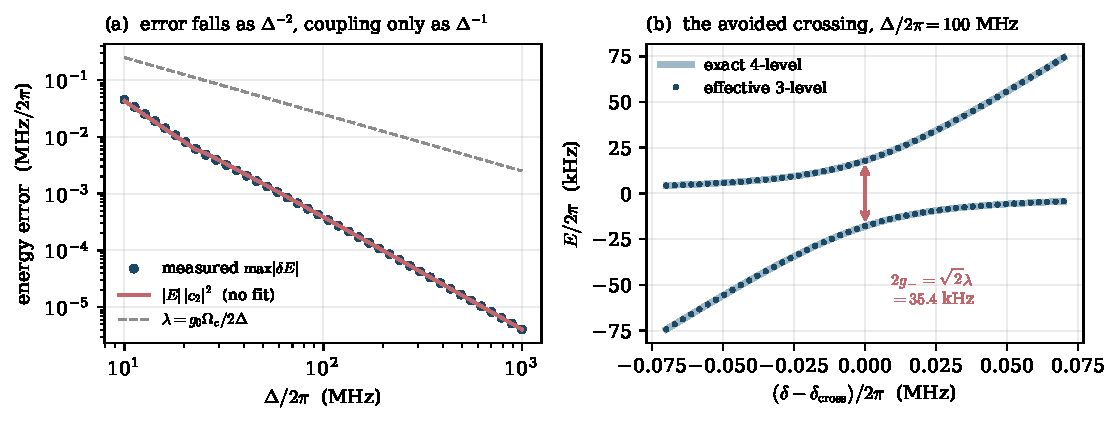
\includegraphics[width=\textwidth]{fig_adiabatic.pdf}
  \caption{\textbf{Step 3 tested against exact diagonalisation} of Eq.~\eqref{eq:Hn} at $n=1$,
  with $g_0/2\pi=1$, $\Om_c/2\pi=5$, $\Omu/2\pi=2$, $\delta/2\pi=0.3$~MHz and $\Dmu=0$.
  \textbf{(a)} Worst-case eigenvalue error against detuning (points), compared with
  Eq.~\eqref{eq:err} (line), which contains no fitted quantity; the Raman coupling $\lambda$ is
  drawn for scale, falling only as $\Delta^{-1}$. \textbf{(b)} The avoided crossing between the
  cavity and the lower dressed branch at $\Delta/2\pi=100$~MHz, whose width is the quantity
  Step~3 exists to produce. Measured minimum gap $35.9$~kHz against the predicted
  $2g_-=\sqrt2\,\lambda=35.4$~kHz; the $1.5\%$ excess is the $\Om_c^2/4\Delta$ light shift,
  which sits on $\ket{3}$ alone and therefore slightly reshapes the dressing of Step~4.}
  \label{fig:adiabatic}
\end{figure}

Collecting the conditions under which the step is justified,
\begin{equation}
  |\Delta| \ \gg\ \Om_c,\quad g_0\sqrt{n},\quad
  \Omu,\quad |\delta|,\quad |\omega_c|,\quad \Gamma_e .
  \tag{A2}
\end{equation}
The first two are the couplings $V_m$ that reach $\ket{2}$; the middle three are the energies
$E$ of the states retained, which is what had to be small beside $\Delta$; the last is the
width of the level removed. All six enter, and the list is worth keeping whole: a treatment that
checks only $|\Delta|\gg\Om_c,\Gamma_e$ will be caught out at large photon number, where
$g_0\sqrt n$ creeps up on $\Delta$. At $\Delta/2\pi=100$ and $g_0/2\pi=1$~MHz the elimination
holds to $n\sim10^3$ and no further.

\begin{keybox}
\textbf{Where the dominant systematic comes from.} The corrections in Eq.~\eqref{eq:pt} are all
built from the same three numbers $V_m$, so they cannot be adjusted independently: the Raman
coupling $\lambda\propto\Om_c$ and the light shift $\propto\Om_c^2$ both track the control-laser
intensity, and the shift adds \emph{directly} to $\delta$ --- the very quantity the measurand
moves. Since $\Om_c^2\propto I$, a fractional intensity fluctuation $\varepsilon$ displaces
$\delta$ by $\varepsilon\,\Om_c^2/4\Delta$, at the numbers above
$\varepsilon\times2\pi\times62$~kHz. Control-laser intensity noise is therefore structurally
indistinguishable from signal, and no amount of care with the microwave will separate them.
\end{keybox}

\section{Step 4: dress the Rydberg pair}

The lower-right block of Eq.~\eqref{eq:H3} is a two-level problem on its own:
\begin{equation}
  H_\mu=\begin{pmatrix}\delta & \Omu/2\\ \Omu/2 & \delta+\Dmu\end{pmatrix}
      = \Bigl(\delta+\tfrac{\Dmu}{2}\Bigr)\mathbf{1}
        + \tfrac12\bigl(\Omu\,\sigma_x + \Dmu\,\sigma_z\bigr).
\end{equation}
Diagonalise with the rotation $R(\theta)$ defined by
\begin{equation}
  \tan\theta = \frac{\Omu}{\Dmu},
  \qquad
  \ket{+} = \sin\tfrac\theta2\ket{3}+\cos\tfrac\theta2\ket{4},
  \qquad
  \ket{-} = \cos\tfrac\theta2\ket{3}-\sin\tfrac\theta2\ket{4},
\end{equation}
giving the \emph{generalised Rabi} splitting
\begin{equation}
  \boxed{\ \omega_\pm=\delta+\frac{\Dmu}{2}\pm\frac{W}{2},
  \qquad W=\sqrt{\Omu^{2}+\Dmu^{2}}\ }
  \label{eq:branches}
\end{equation}
Now rotate the rest of Eq.~\eqref{eq:H3}. The Raman coupling connects $\ket{1}$ to the
\emph{bare} $\ket{3}=\sin\tfrac\theta2\ket{+}+\cos\tfrac\theta2\ket{-}$, so it splits between
the branches in that ratio. In the basis $(\ket{g},\ket{+},\ket{-})$:
\begin{equation}
  \boxed{\;
  H^{(3)}=\begin{pmatrix}
    0 & g_+ a\dg & g_- a\dg\\[3pt]
    g_+ a & \omega_+ & 0\\[3pt]
    g_- a & 0 & \omega_-
  \end{pmatrix},
  \qquad
  g_+=\lambda\sin\tfrac\theta2,\quad g_-=\lambda\cos\tfrac\theta2 \;}
  \label{eq:core}
\end{equation}
There is no $\ket{+}\!\leftrightarrow\!\ket{-}$ entry: that transition is the microwave one and
carries no cavity matrix element.

Equation~\eqref{eq:core} is where this note stops. It is still excitation-number conserving,
so on its own it radiates nothing; turning it into a Dicke model requires counter-rotating
terms $a\dg b\dg+ab$ from a second drive tone, and that, together with the
Holstein--Primakoff step and the superradiant threshold, is the subject of the companion note.


\appendix
\section{The same elimination by hand}
\label{app:hand}

Section~4 eliminated $\ket{2}$ from the eigenvalue problem, which is the right thing to do when
one wants energies. The same elimination can be carried out on the time-dependent problem, where
the assumption being made --- that $\ket{2}$ has no independent motion of its own --- is easier
to see. Expand the state as $\ket{\Psi}=\sum_j\ket{j}\otimes\ket{\phi_j}$ with $\ket{\phi_j}$ (unnormalised) cavity
states. Reading the rows of Eq.~\eqref{eq:H4},
\begin{align}
  i\,\partial_t\ket{\phi_1} &= \omega_c a\dg a\ket{\phi_1} + g_0\,a\dg\ket{\phi_2},
    \label{app:r1}\\
  i\,\partial_t\ket{\phi_2} &= \omega_c a\dg a\ket{\phi_2} + \Delta\ket{\phi_2}
     + g_0\,a\ket{\phi_1} + \tfrac{\Om_c}{2}\ket{\phi_3},
    \label{app:r2}\\
  i\,\partial_t\ket{\phi_3} &= \omega_c a\dg a\ket{\phi_3} + \delta\ket{\phi_3}
     + \tfrac{\Om_c}{2}\ket{\phi_2} + \tfrac{\Omu}{2}\ket{\phi_4},
    \label{app:r3}
\end{align}
and a fourth line for $\ket{\phi_4}$ that never involves $\ket{\phi_2}$. Only
Eq.~\eqref{app:r2} carries a large coefficient. Remove the slow diagonal terms with
$\ket{\phi_j}=e^{-i\omega_c a\dg a\,t}e^{-i\epsilon_j t}\ket{\chi_j}$,
$\epsilon_{1,3,4}=0,\delta,\delta+\Dmu$, and it becomes
\begin{equation}
  i\,\partial_t\ket{\chi_2} = \Delta\ket{\chi_2}
   + \underbrace{g_0\,a\,e^{-i\omega_c t}\ket{\chi_1}
     + \tfrac{\Om_c}{2}e^{-i\delta t}\ket{\chi_3}}_{\textstyle S(t)} ,
\end{equation}
a driven first-order equation whose source has amplitudes $g_0\sqrt{\langle n\rangle}$,
$\Om_c/2$ and turns over at rates $\omega_c,\delta$ --- condition (A2), item by item. When
$|\Delta|$ dominates all of them, $\ket{\chi_2}$ never builds up: it locks to the value that
makes the right-hand side vanish, $\ket{\chi_2}\simeq-S(t)/\Delta$, i.e.
\begin{equation}
  \ket{\phi_2} \;\simeq\; -\frac{1}{\Delta}
    \Bigl(g_0\,a\ket{\phi_1} + \tfrac{\Om_c}{2}\ket{\phi_3}\Bigr).
  \label{app:slave}
\end{equation}
$\ket{2}$ is no longer a degree of freedom; it is a shadow of the two states that drive it.
Substituting into Eq.~\eqref{app:r1},
\begin{equation}
  g_0\,a\dg\ket{\phi_2} = -\frac{g_0^2}{\Delta}\,a\dg a\ket{\phi_1}
      - \frac{g_0\Om_c}{2\Delta}\,a\dg\ket{\phi_3},
\end{equation}
and into Eq.~\eqref{app:r3},
\begin{equation}
  \tfrac{\Om_c}{2}\ket{\phi_2} = -\frac{g_0\Om_c}{2\Delta}\,a\ket{\phi_1}
      - \frac{\Om_c^{2}}{4\Delta}\ket{\phi_3}.
\end{equation}
These are the same four paths tabulated in \S\ref{sec:paths}, and they assemble into the same
Eq.~\eqref{eq:H3}. The correspondence with \S4.2 is exact: Eq.~\eqref{app:slave} is
Eq.~\eqref{eq:c2} with $E$ already dropped from the denominator, and substituting it back into
the remaining rows multiplies it by $V_m$, which is Eq.~\eqref{eq:pt}. The two calculations
answer different questions --- one the stationary energies, the other the motion of an arbitrary
state --- and make the same single approximation.

\end{document}
